\documentclass[11pt]{article}
\usepackage[margin=1in]{geometry}
\usepackage[T1]{fontenc}
\usepackage[utf8]{inputenc}
\usepackage{graphicx}
\usepackage{booktabs}
\usepackage{tabularx}
\usepackage{array}
\usepackage{float}
\usepackage{hyperref}
\usepackage{xcolor}
\usepackage{listings}

\hypersetup{
  colorlinks=true,
  linkcolor=blue,
  urlcolor=blue,
  citecolor=blue
}

\setlength{\parindent}{0pt}
\setlength{\parskip}{0.6em}

\title{Tech Titans\\Milestone 5 Report\\Incremental Draft: Experiments 1 and 2}
\author{CMPT 470/816\\Assigned Repository: Gson}
\date{March 30, 2026}

\begin{document}
\maketitle

\textbf{Draft scope.} This report revision documents only Milestone 5 Experiments 1 and 2 using recorded local runs. Experiments 3--5 will be added in later revisions; no placeholder results are claimed here.

\section{Introduction}
Mutation testing measures whether a test suite can detect seeded faults rather than merely execute the corresponding lines. For Milestone 5, our goal is to use PIT on Gson to assess the quality of tests around a coherent parsing and streaming subsystem, document the setup process, and establish a reproducible baseline before deeper surviving-mutant analysis in later experiments.

This draft focuses on two questions. First, can PIT be configured reproducibly on Gson with a justified and non-trivial target scope? Second, once that scope is fixed, what does the first full mutation baseline reveal about the current test suite? The emphasis in this revision is therefore on configuration, scope calibration, and accurate baseline reporting from real runs.

\section{Background}
Mutation testing works by generating small source-level or bytecode-level changes, running the existing tests, and classifying each mutant as killed, survived, not covered, or timed out. Unlike line coverage, mutation results say something about the strength of the assertions and the sensitivity of the tests to behavior changes. A project can execute nearly all lines in a subsystem and still allow important mutants to survive.

PIT is a practical Java mutation testing tool because it performs coverage analysis first and only runs tests relevant to each mutant. It also produces HTML and XML reports that expose both high-level project metrics and per-mutant details. This matters for Gson because the selected scope contains both deeply stateful parsing code and smaller adapter or bridge classes. Those classes are all part of one feature area, but they differ substantially in how much mutatable logic they contain.

Equivalent mutants remain a known limitation. A mutant can survive either because tests are weak or because the mutated program is behaviorally indistinguishable from the original. Distinguishing those cases is part of later milestone work, but even in Experiments 1 and 2 it is important to avoid over-interpreting raw survival counts.

\section{Experimental Setup}
\subsection{Dataset Declaration}
\begin{table}[H]
\centering
\small
\begin{tabularx}{\linewidth}{>{\raggedright\arraybackslash}p{0.28\linewidth}X}
\toprule
Item & Value \\
\midrule
Group & Tech Titans \\
Repository & Gson \\
Repository URL & \url{https://github.com/google/gson.git} \\
Commit used & \texttt{1fa9b7a0a994b006b3be00e2df9de778e71e6807} \\
Build module & \texttt{gson/gson} \\
Declared \texttt{targetClasses} &
\texttt{com.google.gson.stream.*},
\texttt{com.google.gson.JsonStreamParser},
\texttt{com.google.gson.JsonParser},
\texttt{com.google.gson.internal.Streams},
\texttt{com.google.gson.internal.bind.JsonTreeReader},
\texttt{com.google.gson.internal.bind.JsonTreeWriter},
\texttt{com.google.gson.internal.bind.JsonElementTypeAdapter} \\
Declared \texttt{targetTests} & \texttt{com.google.gson.*} \\
Approximate selected source LOC & 4,201 raw lines across 12 selected source files \\
PIT mutated-class LOC in final baseline & 1,361 lines reported by PIT \\
Total test cases in scope & 4,586 tests in the green-suite validation run \\
\bottomrule
\end{tabularx}
\caption{Dataset declaration for the selected Gson mutation-testing scope.}
\end{table}

\subsection{Scope Selection, Justification, and Hypothesis}
The selected scope expands outward from Gson's streaming subsystem rather than redirecting the analysis to a different part of the project. The core package \texttt{com.google.gson.stream} contains the most stateful reader and writer logic in the chosen slice, especially \texttt{JsonReader} and \texttt{JsonWriter}. We then added adjacent parser and tree-bridge classes that sit directly on top of that streaming layer: \texttt{JsonParser}, \texttt{JsonStreamParser}, \texttt{Streams}, \texttt{JsonTreeReader}, \texttt{JsonTreeWriter}, and \texttt{JsonElementTypeAdapter}.

This is a feature-based selection. The classes together implement one coherent concern: parsing JSON text or trees, traversing it, and serializing it back out. The scope is also complexity-oriented. The reader/writer classes are state machines with many branching conditions, while the tree bridge classes expose smaller but still meaningful control-flow decisions around adapter behavior, null handling, and reader/writer transitions.

Before running the full baseline, our hypothesis was that this subsystem would show very high line coverage and a moderately high mutation score because Gson already ships dedicated reader, writer, parser, and tree-adapter tests. We nevertheless expected some surviving mutants in control-flow edges, leniency handling, and return-value behavior, especially in the bridge classes where tests are often more scenario-driven than assertion-heavy.

\subsection{Environment and PIT Configuration}
\begin{table}[H]
\centering
\small
\begin{tabularx}{\linewidth}{>{\raggedright\arraybackslash}p{0.34\linewidth}X}
\toprule
Item & Value \\
\midrule
PIT version & 1.15.3 \\
Build tool & Apache Maven 3.9.11 \\
Java version & Eclipse Temurin 17.0.17 \\
Operating system & Linux 6.12.5-linuxkit on \texttt{aarch64} \\
Mutation operators & \texttt{DEFAULTS} \\
Report formats & HTML and XML \\
Threads & 7 \\
Timeout constant & 5000 ms \\
JVM max heap & \texttt{-Xmx1024m} \\
History mode & Disabled (\texttt{withHistory=false}) \\
Excluded test classes & \texttt{com.google.gson.integration.*} \\
Test plugin note & No separate \texttt{pitest-junit5-plugin} was configured; this project uses JUnit 4 tests \\
\bottomrule
\end{tabularx}
\caption{Execution environment and key PIT parameters.}
\end{table}

The PIT configuration is defined in the Maven profile \texttt{milestone5-pit}. All default mutators were enabled, and PIT produced both HTML and XML reports as required. The full configuration excerpt is included in Appendix A.

\subsection{Pre-run Validation and Setup Challenges}
We first validated that the selected module had a green test suite before any mutation run. The Docker-based verification run completed successfully with 4,586 tests executed, 0 failures, 0 errors, and 19 skipped tests in 38.081 seconds. This satisfied the milestone requirement to confirm a passing suite before PIT.

To verify the PIT configuration itself, we then performed a smoke run on the original streaming slice, namely \texttt{com.google.gson.stream.*} together with \texttt{com.google.gson.JsonStreamParser}. This was intentionally used as a calibration step because it is the narrowest coherent subset of the final scope and exercises the same parser/streaming behavior. The smoke run produced a valid HTML report, generated 687 mutants, and completed in 55 seconds of PIT time (1 minute 10 seconds wall-clock through Maven), which is in the assignment's marginal range and therefore suggested that the scope could be widened further.

\begin{figure}[H]
\centering
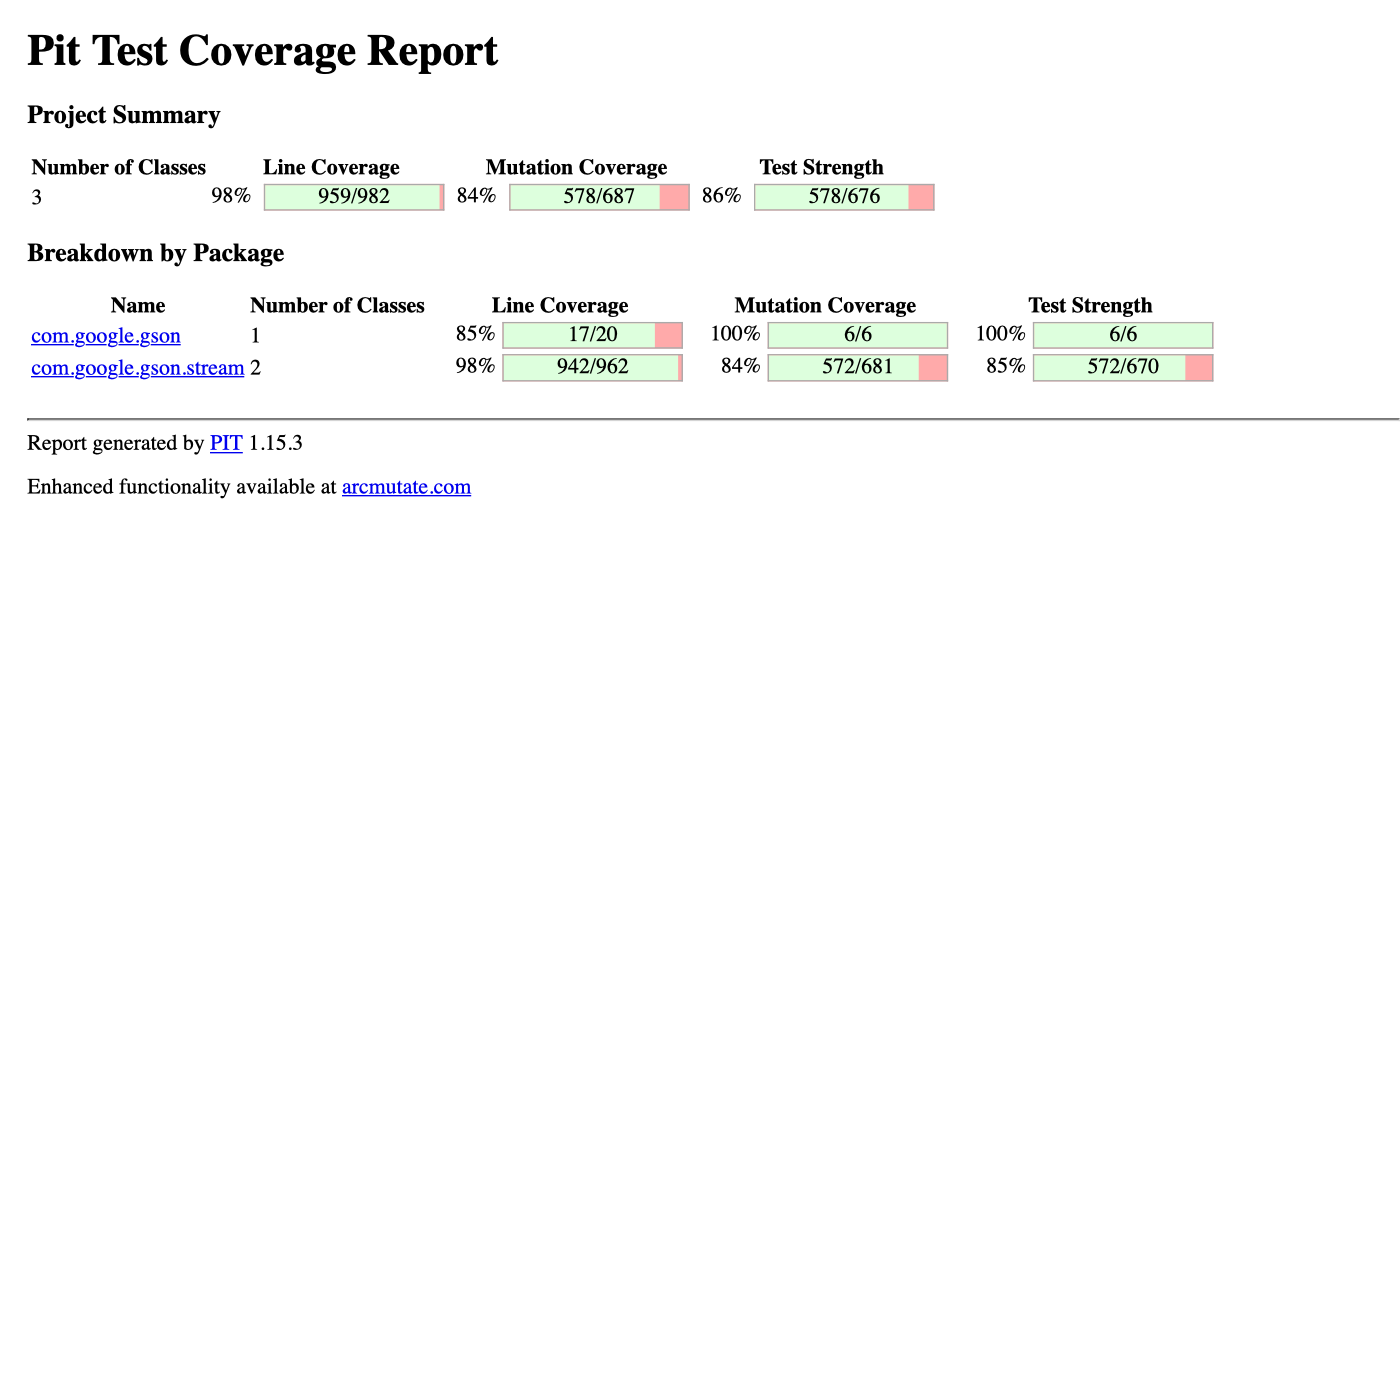
\includegraphics[width=0.88\linewidth]{figures/pit-smoke-report.png}
\caption{Smoke-run HTML report rendered from the recorded PIT artifact for setup verification.}
\end{figure}

Two practical setup issues mattered. First, Gson must be executed from the inner module directory \texttt{gson/gson}; running PIT from the repository root would not target the actual library module under test. Second, the initial streaming-only selection contained several files that were in scope but effectively non-mutatable under PIT defaults, including constant-only or metadata-only files. Because that reduced the effective mutatable surface and kept runtime low, we expanded the scope to adjacent parser/tree classes while preserving the same subsystem focus. This calibration step moved the final baseline runtime into the milestone's preferred 2--30 minute band.

\section{Results}
\subsection{Experiment 1: PIT Setup and Configuration}
Experiment 1 succeeded on all required points: PIT was installed in Maven, the selected target patterns were documented, default mutators were enabled, HTML and XML outputs were generated, the full test suite passed before mutation analysis, and a smoke PIT run produced a valid report.

The smoke run also provided the first empirical scope-calibration signal. Although the streaming slice was logically coherent, PIT reported only 982 mutated-class LOC despite 3,038 raw source lines in the declared selection. Investigation of the smoke report showed that this happened because some selected files such as \texttt{JsonToken}, \texttt{JsonScope}, \texttt{MalformedJsonException}, and \texttt{package-info.java} contributed little or no mutatable logic under PIT defaults. That observation directly motivated the expanded final scope.

\begin{table}[H]
\centering
\small
\begin{tabularx}{\linewidth}{>{\raggedright\arraybackslash}p{0.38\linewidth}X}
\toprule
Smoke-run metric & Observed value \\
\midrule
Declared smoke scope & \texttt{com.google.gson.stream.*} and \texttt{com.google.gson.JsonStreamParser} \\
Raw selected source LOC & 3,038 \\
PIT mutated-class LOC & 982 \\
Generated mutants & 687 \\
Killed mutants & 572 \\
Survived mutants & 98 \\
Timed-out mutants & 6 \\
No-coverage mutants & 11 \\
Mutation score & 85.4\% \\
PIT test strength & 86\% \\
Line coverage & 98\% \\
Runtime & 55 seconds PIT time; 1 minute 10 seconds Maven wall-clock \\
\bottomrule
\end{tabularx}
\caption{Experiment 1 smoke-run results, computed from the recorded PIT HTML/XML artifacts and log.}
\end{table}

\subsection{Experiment 2: Full Mutation Analysis}
After calibration, the final expanded scope produced a substantially stronger baseline while remaining tightly focused on the same subsystem. The baseline report covers eight PIT-mutated classes distributed across the Gson streaming, parser, internal bridge, and tree-adapter packages. In raw source terms the declared scope spans 4,201 lines across 12 selected source files; in PIT's own project summary, the effective mutated-class footprint is 1,361 lines.

\begin{table}[H]
\centering
\small
\begin{tabular}{lrrrrrrrr}
\toprule
Project & LOC & Tests & Mutants & Killed & Surv. & No Cov. & Mut. Score & Test Str. \\
\midrule
Gson selected scope & 4201 & 4586 & 945 & 786 & 132 & 18 & 85.6\% & 86\% \\
\bottomrule
\end{tabular}
\caption{Milestone 5 summary table for the full Experiment 2 baseline. Timed-out mutants: 9; line coverage: 96\%; runtime: 4 minutes 9 seconds wall-clock.}
\end{table}

The final baseline generated 945 mutants and killed 786 of them, with 132 surviving, 18 not covered, and 9 timing out. Using the milestone formula, the mutation score is therefore $786 / (786 + 132) = 85.6\%$. PIT's HTML summary also reports 84\% mutation coverage and 86\% test strength. The difference is expected: PIT's top-line mutation coverage counts timed-out mutants as detected and normalizes differently from the milestone's explicit mutation-score formula.

Line coverage remained high at 1,309/1,361 mutated-class lines (96\%), and the runtime increased to 4 minutes 9 seconds wall-clock, which places the final selected scope squarely in the assignment's preferred execution range. PIT executed 14,461 relevant test invocations during mutation analysis, while the green-suite validation established that the total test suite in scope contains 4,586 test cases.

\begin{table}[H]
\centering
\footnotesize
\begin{tabularx}{\linewidth}{>{\raggedright\arraybackslash}p{0.33\linewidth}rrrrrr}
\toprule
Operator & Generated & Killed & Survived & Timed Out & No Cov. & Kill Rate \\
\midrule
\texttt{RemoveConditionalMutator\_EQUAL\_ELSE} & 343 & 298 & 39 & 3 & 3 & 88.4\% \\
\texttt{MathMutator} & 179 & 145 & 30 & 2 & 2 & 82.9\% \\
\texttt{VoidMethodCallMutator} & 131 & 119 & 7 & 1 & 4 & 94.4\% \\
\texttt{NullReturnValsMutator} & 85 & 54 & 25 & 0 & 6 & 68.4\% \\
\bottomrule
\end{tabularx}
\caption{Top four mutation operators by generated mutant count in the Experiment 2 baseline. Kill rate is computed as killed / (killed + survived), with timed-out mutants reported separately.}
\end{table}

The operator breakdown highlights two patterns. First, most of the mutant volume comes from control-flow and arithmetic rewrites inside the reader/writer state machines, which is consistent with the scope selection. Second, \texttt{NullReturnValsMutator} has the weakest kill rate among the four largest operators, which suggests that return-value assertions around some bridge or fluent API paths are weaker than branch assertions in the core parsing logic.

\section{Discussion}
The full baseline largely confirmed the pre-run hypothesis. The selected Gson subsystem has very high line coverage and a strong overall mutation score, which indicates that the existing test suite is not merely executing code but is detecting many seeded faults. That is especially clear in the streaming layer, where \texttt{JsonReader} and \texttt{JsonWriter} account for most mutants and are still tested strongly.

At the same time, the calibration step mattered. The original streaming-only selection was coherent but too narrow in effective mutatable surface because several selected files were trivial under PIT's default mutators. Expanding to adjacent parser and tree-bridge classes preserved the architectural focus while improving experimental value. The final 4:09 runtime is much more appropriate for the milestone than the 55-second smoke run.

The results also show why mutation testing gives a different picture from coverage alone. Even with 96\% mutated-class line coverage, 132 mutants survived in the final baseline. That gap is exactly why later experiments need to inspect surviving mutants rather than stop at the summary numbers. For now, the baseline already points to promising areas for deeper analysis: return values, arithmetic/state transitions, and conditional rewrites in tree-bridge or parser-edge behavior.

\section{Lessons Learned}
Three lessons are already clear from Experiments 1 and 2. First, scope selection must be guided by mutatable logic rather than raw source lines alone. Second, a subsystem-focused scope can stay small enough to run repeatedly while still generating nearly a thousand mutants if the selected classes actually contain branching behavior. Third, high coverage by itself would have overstated test adequacy; the surviving mutants show that substantial room for improvement remains even in a well-tested library.

\section{Conclusion}
For this selected Gson subsystem, PIT setup was reproducible and the final baseline produced a useful mutation-testing workload: 945 mutants, 85.6\% mutation score by the milestone formula, 86\% PIT test strength, 96\% line coverage, and a 4:09 wall-clock runtime. These results suggest that mutation testing is practical and informative for a production Java project when the scope is chosen as a coherent feature slice with meaningful logic and a runtime in the low-minute range.

The next report revisions will build on this baseline by analyzing specific surviving mutants, evaluating operator effectiveness in more depth, and measuring score sensitivity under targeted test changes. Those later experiments will reuse the same repository and the same final target scope documented here.

\appendix
\section{PIT Configuration Excerpt}
\begin{lstlisting}[basicstyle=\ttfamily\small,breaklines=true]
<profile>
  <id>milestone5-pit</id>
  <properties>
    <pitest.version>1.15.3</pitest.version>
    <pitest.target.tests>com.google.gson.*</pitest.target.tests>
    <pitest.target.class.1>com.google.gson.stream.*</pitest.target.class.1>
    <pitest.target.class.2>com.google.gson.JsonStreamParser</pitest.target.class.2>
    <pitest.target.class.3>com.google.gson.JsonParser</pitest.target.class.3>
    <pitest.target.class.4>com.google.gson.internal.Streams</pitest.target.class.4>
    <pitest.target.class.5>com.google.gson.internal.bind.JsonTreeReader</pitest.target.class.5>
    <pitest.target.class.6>com.google.gson.internal.bind.JsonTreeWriter</pitest.target.class.6>
    <pitest.target.class.7>com.google.gson.internal.bind.JsonElementTypeAdapter</pitest.target.class.7>
    <pitest.threads>7</pitest.threads>
    <pitest.timeout.constant>5000</pitest.timeout.constant>
    <pitest.withHistory>false</pitest.withHistory>
    <pitest.jvm.maxHeap>1024m</pitest.jvm.maxHeap>
  </properties>
  <build>
    <plugins>
      <plugin>
        <groupId>org.pitest</groupId>
        <artifactId>pitest-maven</artifactId>
        <version>${pitest.version}</version>
        <configuration>
          <targetClasses>
            <param>${pitest.target.class.1}</param>
            <param>${pitest.target.class.2}</param>
            <param>${pitest.target.class.3}</param>
            <param>${pitest.target.class.4}</param>
            <param>${pitest.target.class.5}</param>
            <param>${pitest.target.class.6}</param>
            <param>${pitest.target.class.7}</param>
          </targetClasses>
          <targetTests>
            <param>${pitest.target.tests}</param>
          </targetTests>
          <excludedTestClasses>
            <param>com.google.gson.integration.*</param>
          </excludedTestClasses>
          <mutators>
            <mutator>DEFAULTS</mutator>
          </mutators>
          <outputFormats>
            <param>HTML</param>
            <param>XML</param>
          </outputFormats>
          <jvmArgs>
            <value>-Xmx${pitest.jvm.maxHeap}</value>
          </jvmArgs>
          <withHistory>${pitest.withHistory}</withHistory>
          <timestampedReports>false</timestampedReports>
          <failWhenNoMutations>true</failWhenNoMutations>
        </configuration>
      </plugin>
    </plugins>
  </build>
</profile>
\end{lstlisting}

\section{Artifact Locations Used in This Draft}
\begin{itemize}
  \item Green-suite verification log: \url{logs/verify-gson-docker.log}
  \item PIT smoke log: \url{logs/pit-smoke-docker.log}
  \item PIT smoke reports: \url{artifacts/pit/smoke/index.html} and \url{artifacts/pit/smoke/mutations.xml}
  \item PIT baseline log: \url{logs/pit-baseline-docker.log}
  \item PIT baseline reports: \url{artifacts/pit/baseline/index.html} and \url{artifacts/pit/baseline/mutations.xml}
  \item PIT Maven profile: \url{gson/gson/pom.xml}
\end{itemize}

\end{document}
